\documentclass[onecolumn,           % Format : preprint, twocolumn
%\documentclass[preprint,           % Format : preprint, twocolumn
               showpacs,            % Pacs : showpacs, noshowpacs
               preprintnumbers,     % Preprint: preprintnumbers,
               			    %           nopreprintnumbers
               aps,                 % Society: ...
               prl,          	    % Journal Style : pra, prb, prc, prd, pre,
               			    %                 prl, prstab, rmp
               letterpaper,             % Size : a4paper, ...
               superscriptaddress,      % Affiliation (Title) : groupedaddress,
                                    %                       superscriptaddress,
                                    %                       unsortedaddress
               nofootinbib,         % Footnote: footinbib, nofootinbib
               tightenlines,        % Remove additional spaces in a line
               floats,floatfix      % Floating pictures and tables
               ,usenatbib,
               ]{revtex4-1}
\usepackage{graphicx}  % needed for figures
\usepackage{dcolumn}   % needed for some tables}
%\usepackage[style=authoryear,backend=biber]{biblatex}
\usepackage{bm}        % for math
\usepackage{amsmath,amssymb}
\usepackage{hyperref}
\usepackage{color}
\definecolor{purple}{rgb}{0.58,0.0,0.83}
\usepackage{caption}
\usepackage[toc,page]{appendix}

\begin{document}

\title{ESTAD\'ISTICA BAYESIANA Y COSMOLOG\'IA}
\begin{abstract}
XX\\
XX\\
XX\\
XX\\
XX\\
XX\\
XX\\
XX\\
\end{abstract}

\maketitle
\section{Estad\'istica Bayesiana vs Frecuentista}

Antes de comenzar nuestra incursi\'on a trav\'es del mundo de un estad\'istico Bayesiano es importante conocer cuales son las principales diferencias que distinguen un pensamiento Bayesiano de uno Frecuentista. As\'i pues, en esta secci\'on introducieron estas discrepancias, analizando las consecuencias desprendidas de estos conceptos.

Comenzaremos definiendo el concepto m\'as importante para cualquier procedimiento estad\'istico, esto es, el concepto de probabilidad. Si consideramos que $x$ es una variable aleatoria relacionada con un evento en particular y $P(x)$ su probabilidad correspondiente, entonces para ambos casos se debe cumplir que
\begin{subequations}\label{axiomas}
\begin{equation}\label{1a}
P(x)\geq 0,
\end{equation}
\begin{equation}\label{1b}
\int_{-\infty}^\infty dxP(x) = 1.
\end{equation}
Para eventos mutuamente excluyentes,
\begin{equation}\label{1c}
P(x_1 \cup x_2) = P(x_1)+P(x_2), \ \ \ \ \text{si }x_1\cap x_2 = \emptyset
\end{equation}
En general
\begin{equation}\label{1d}
P(x_1,x_2) = P(x_1)P(x_1|x_2)
\end{equation}
\end{subequations}
En palabras, la \'ultima regla nos dice que la probabilidad de que $x_1$ y $x_2$ pasen estar\'a dada por el producto entre la probabilidad de que $x_1$ pase con la probabilidad condicional de que $x_2$ pase tal que $x_1$ ha pasado.

Y entonces, ?`en qu\'e consiste la diferencia entre ambas disciplinas? B\'asicamente, la diferencia principal entre la estad\'istica Bayesiana y la Frecuentista consiste  en su definici\'on de probabilidad. En la estad\'istica frecuentista, \textbf{probabilidad est\'a fundamentalmente relacionada con una frecuencia de eventos}, i.e. $p=n/N$, donde $n$ es el numero de sucesos de un evento, mientras que $N$ es el n\'umero total de intentos. Por otro lado, en la estad\'istica Bayesiana, \textbf{probabilidad es fundamentalmente relacionada con nuestro propio conocimiento sobre alg\'un evento}.

Ahora bien, cualquier procedimiento estad\'istico  conciste de 3 ingredientes b\'asicos que deben ser entendidos dependiendo el tipo de estad\'istica que estemos empleando:  los datos, el modelo y un m\'etodo de estimaci\'on.

\textit{Los datos} son una medida de nuestras observaciones, los cuales denotaremos como $D$. Para un estad\'istico Frecuentista, dichos datos son el producto de un evento repetible, mientras que para uno Bayesiano los datos se observan a partir de una muestra realizada, no necesariamente repetible, por lo que estos deben tomarse fijos para el an\'alisis estad\'istico.

Luego tenemos el modelo. Este concepto difiere dependiendo de que interpretaci\'on estad\'istica estemos utilizando. En general, un \textit{modelo}, $Q$, es una colecci\'on de mediciones de probabilidades $P$. Las distribuciones $P_\theta$ son llamadas distribuciones del modelo, donde $\theta$ son aquellos par\'ametros que $Q$ contiene. La diferencia entre ambas clases de estad\'siticas recae en el valor que los par\'ametros $\theta$ pueden tener. Mientras que para un pensamiento frecuentista los par\'ametros $\theta$ son fijos y existe s\'olo un valor del par\'ametro $\theta_0$ al que nuestros datos pertenecen, para un pensamiento Bayesiano los par\'ametros $\theta$ no poseen un \'unico valor. De hecho, en la estad\'istica Bayesiana, se considera que no existe diferencia matem\'atica formal entre par\'ametros y datos, por lo que para ambos casos se debe asociar una distribuci\'on de probabilidad.

Finalmente nos encontramos con el estimador de $P_0$. Un estimador para $P_0$ es la representaci\'on de nuestra ``mejor creencia" de $P$ dados los datos $D$, i.e. $P_0 = P_{mejor}$. 

De esta manera en la tabla \ref{table:1} podemos resumir las principales diferencias entre ambas estad\'isticas. 

\begin{table}[h!]
\centering
\begin{tabular}{||l|l||} 
 \hline
 \textbf{Frecuentista} & \textbf{Bayesiano} \\ [0.5ex] 
 \hline\hline
 Los datos son una muestra aleatoria  & Los datos son observados a partir de la  \\ 
 repetible. Existe una frecuencia de eventos. &muestra realizada. \\
 \hline 
Los par\'ametros del modelo se mantienen& Los par\'ametros son desconocidos y deben ser \\
 constantes durante este proceso repetible. & descritos probabil\'isticamente. \\
\hline
Los par\'ametros se toman fijos. & Los datos se toman fijos.\\ [1ex] 
 \hline
\end{tabular}
\caption{\footnotesize{Principales diferencias entre las interpretacion Frecuentista y la Bayesiana.}}
\label{table:1}
\end{table}

\section{Introducci\'on a la Estad\'istica Bayesiana}

En esta secci\'on introduciremos brevemente los conceptos matem\'aticos b\'asicos que son necesarios para poder emplear el formalismo Bayesiano a la cosmolog\'ia. Posteriormente, en la siguiente secci\'on nos concentraremos en las herramientas computacionales que nos ayudar\'an a simplificarnos la vida cuando un an\'alisis anal\'itico no sea posible (que ser\'a pr\'acticamente en todos los casos). 

\subsection{Teorema de Bayes, priors, posteriores y esas cosas}

El tratamiento Bayesiano a un problema estad\'istico siempre estar\'a centrado en lo que es conocido como el teorema de Bayes. Este teorema es una concecuencia directa de los axiomas de la probabilidad \eqref{axiomas}. Podemos observar de \eqref{1c}, sin p\'erdida de generalidad, que siempre es posible reescribir $P(x_2,x_1)=P(x_2)P(x_2|x_1)$. Luego, como es de esperarse que la relaci\'on $P(x_1,x_2)=P(x_2,x_1)$ se cumpla, obtenemos que
\begin{equation}
P(x_2|x_1)=\frac{P(x_2)P(x_1|x_2)}{P(x_1)}.
\end{equation}
Este \'ultimo resultado es conocido como el \textit{teorema de Bayes}. Por otro lado, ya que hab\'iamos mencionado anteriormente que en la estad\'istica Bayesiana no existe distinci\'on formal entre datos y par\'ametros, podemos reescribir la ecuaci\'on anterior haciendo los cambios $x_1\rightarrow D$ y $x_2\rightarrow H$, como
\begin{equation}\label{BayesT}
P(\theta,H|D)=\frac{P(\theta,H)P(D|\theta,H)}{P(D)}
\end{equation}
En esta expresi\'on hemos agregado el t\'ermino extra $\theta$ para especificar que $H$ depende de dichos par\'ametros. Por otro lado, notemos que hemos agregado una nueva cantidad $H$, que llamaremos nuestra ``hip\'otesis". Esta \'ultima corresponde al modelo $Q$ que seg\'un nuestra creencia mejor se ajustar\'ia a los datos, i.e. $H=Q_{mejor}$.

Notemos que ahora, de la expresi\'on anterior, contamos con 4 nuevos entes que deben ser entendidos a la perfecci\'on antes de poder continuar con este cap\'itulo.  En primera instancia $P(\theta,H|D)$ es conocida como la distribuci\'on posterior de probabilidad (o s\'implemente posterior). Esta cantidad es b\'asicamente el resultado pr\'incipal a obtener ya que nos habla sobre la probabilidad de nuestro modelo (o par\'ametros del modelo), tal que hemos obtenido cierto conjunto de datos $D$. Usualmente, dicha cantidad es utilizada para acotar los par\'ametros del modelo. Luego tenemos los denominados ``priors", $P(\theta,H)$, los cuales son una distribuci\'on de probabilidad para nuestros par\'ametros, definidos a partir de nuestro propio conocimiento acerca del modelo. Generalmente, en el l\'imite donde tenemos muchos datos, estos priors no son estad\'isticamente importantes, por lo que un prior t\'ipico a tomar para cada par\'ametro del modelo es uno plano (una distribuci\'on uniforme). A continuaci\'on tenemos lo que es conocido como el Likelihood $L(D;\theta)\equiv P(D|\theta,H)$ y es b\'asicamente el elemento m\'as importante al momento de hacer un estudio estad\'istico para la inferencia de los par\'ametros de nuestro modelo. Nos concentraremos en este elemento m\'as adelante. Finalmente nos encontramos con la evidencia Bayesiana (o s\'implemente evidencia). Podemos notar que \'esta act\'ua como un factor de normalizaci\'on
\begin{equation}\label{BayesT}
P(D) = \int d\theta P(\theta,H)P(D|\theta,H).
\end{equation}
De esta manera, esta cantidad es usualmente ignorada cuando el espacio de par\'ametros de un \'unico modelo es probado. Por otro lado, esta cantidad resulta ser fundamental si lo que se quiere es hacer una comparaci\'on entre modelos. Sin embargo, para los prop\'ositos de este cap\'itulo, no nos interesaremos en calcular $P(D)$.

Podemos ver que el teorema de Bayes tiene una implicaci\'on enorme respecto a una inferencia (de par\'ametros, por ejemplo) desde el punto de vista Bayesiano. En un escenario t\'ipico podemos tomar un conjunto de datos y esperar interpretarlos en t\'erminos de alg\'un modelo. Sin embargo, lo que usualmente podemos hacer es lo opuesto, es decir, podemos tener un conjunto de datos y posteriormente confrontar un modelo tomando en cuenta la probabilidad que nuestro modelo se ajuste a los datos. De esta manera, como se puede ver de \eqref{BayesT}, el teorema de Bayes nos permite relacionar ambos escenarios, dandonos la posibilidad de conocer cual es el modelo (o par\'ametros del modelo) que mejor se ajusta a los datos.

\subsection{?` Y qu\'e hay acerca del Likelihood?}

Nuevamente tomando el teorema de Bayes \eqref{BayesT}, si ignoramos la evidencia Bayesiana y consideramos un prior uniforme, el c\'alculo del posterior estar\'a \'unicamente determinado por maximizar el Likelihood. Por supuesto, el ignorar la evidencia ocasiona que no sea posible el poder dar una probabilidad absoluta de los par\'ametros de nuestro modelo, sin embargo, lo que s\'i podemos hacer es dar una probabilidad relativa definida como el cociente entre probabilidades. De esta manera, el Likelihood en un punto particular en el espacio de par\'ametros puede ser comparado con el que mejor se ajuste a las observaciones, $L_{max}$. Podemos decir entonces que un modelo es aceptable si el cociente de los Likelihoods
\begin{equation}
\Lambda=-2\ln\left[\frac{L(D;\theta,H)}{L_{max}}\right]
\end{equation}
es mayor que alg\'un n\'umero dado.

Por otra parte, notemos que si nuestro posterior posee un \'unico m\'aximo global en $\theta_0$, siempre es posible hacer una expansi\'on en serie de la forma
\begin{equation}
\ln L(D;H)=\ln L(D;H_0)+\frac{1}{2}(\theta_\alpha-\theta_{0\alpha})\frac{\partial^2\ln L}{\partial\theta_\alpha \partial\theta_\beta}(\theta_\beta-\theta_{0\beta})+...
\end{equation}
donde $H_0$ corresponde al modelo con los par\'ametros que mejor se ajustan a los datos y $\theta_{0\alpha}$ son los componentes del vector de par\'maetros $\theta_0$.

De esta manera, para estos casos podemos reescribir nuestro Likelihood como
\begin{equation}\label{GLik}
L(D;H)=L(D;H_0)\exp \left[-\frac{1}{2}(\theta_\alpha-\theta_{0\alpha})H_{\alpha\beta}(\theta_\beta-\theta_{0\beta})\right]
\end{equation}
donde
\begin{equation}
H_{\alpha\beta}=\frac{\partial^2\ln L}{\partial\theta_\alpha \partial\theta_\beta}
\end{equation}
es llamada la matriz Hessiana y controla si la estimaci\'on de $\theta_\alpha$ y $\theta_\beta$ se encuentran correlacionadas. Si esta es diagonal, se dice que las estimaciones no est\'an correlacionadas.

Aqu\'i es preciso remarcar que esta aproximaci\'on es buena siempre que contemos con un \'unico m\'aximo global en nuestro posterior. Si por el contrario \'este poseiera m\'ultiples m\'aximos locales, entonces la aproximaci\'on no servir\'ia.

\subsection{Actualizando los posteriores}

Una pregunta natural que puede surgir al momento de hacer cualquier an\'alisis Bayesiano es: ?`qu\'e pasa cuando obtengo nuevos datos? es decir, ?`puedo hacer uso de la informaci\'on que ya conoc\'ia o es preciso volver a calcular todo tomando como mi conjunto de datos los datos viejos m\'as los nuevos? Como [referencias] explica, siempre que los datos sean consistentes entre ellos, no importa cual sea la manera que se elija para analizar los datos, i.e. da lo mismo si primero se utilizan los datos viejos para obtener un posterior y luego dicho posterior se utiliza como prior para analizar los datos nuevos, que tomar el conjunto completo de datos y analizarlos con un prior inicial, digamos uno no informativo (plano).

\subsection{Chi-cuadrada}

Como se coment\'o anteriormente, la forma precisa para encontrar el posterior de alg\'un modelo en particular estar\'a dado por maximizar el Likelihood. Notemos que en la aproximaci\'on gaussiana, dicho tarea es equivalente a minimizar la expresi\'on 
\begin{equation}\label{chi2}
\chi^2\equiv(\theta_\alpha-\theta_{0\alpha})H_{\alpha\beta}(\theta_\beta-\theta_{0\beta}).
\end{equation}
La cantidad $\chi^2$ es usualmente llamada \textit{chi-cuadrada} y se relaciona con el Likelihood Gaussiano v\'ia $L=L_0^{-\chi^2/2}$. As\'i pues, podemos decir que el proceso de maximizar un Likelihood Gaussiano con el de minimizar un chi-cuadrada son equivalentes. Sin embargo, en las circunstancias donde un Likelihood no pueda ser bien especificado por una distribuci\'on gaussiana, entonces ambos procesos ser\'an totalmente distintos.

\subsection{Curvas de contorno y regiones de confidencia}

Una vez que se han obtenido los par\'ametros que mejor se ajustan a los datos, lo que nos gustar\'ia saber es si hay regiones de confidencia donde otros par\'ametros pueden ser considerados como buenos candidatos para nuestro modelo. Una elecci\'on natural ser\'ia considerar regiones donde $\chi^2$ es menor que alg\'un cierto valor dado. Para el caso de distribuciones Gaussianas multi-variadas, como es el caso de \eqref{GLik}, dichas regiones corresponden con elipsoides.

La forma en la que estas regiones de confidencia pueden ser calculadas es un poco t\'ecnica para los fines de este cap\'itulo, sin embargo, para los lectores interesados se les recomienda revisar las referencias [ref].
\subsection{Marginalizaci\'on}

Se puede dar el caso en el que al realizar un experimento s\'olo estemos interesados en analizar ciertos par\'ametros de nuestro modelo o existan par\'ametros extras considerados como ruido. Un ejemplo de estos par\'ametros de ruido podr\'ia ser aquellos correspondientes a efectos de calibraci\'on del experimento. Si este es el caso, lo que usualmente se hace es marginalizar sobre los par\'ametros que no son de inter\'es mediante la expresi\'on
\begin{equation}
P(\theta_1,...,\theta_j,H|D)=\int d\theta_{j+1}...d\theta_{m}P(\theta,H|D)
\end{equation}
donde $m$ es el n\'umero total de par\'ametros en nuestro modelo y $\theta_1,...,\theta_j$ corresponden a los par\'ametros en los que estamos interesados.

\section{M\'etodos Num\'ericos}

En un escenario t\'ipico casi nunca es posible hacer el c\'alculo del posterior de manera anal\'itica. Para estas circunstancias existen toda una cajara de herramientas computacionales que pueden ayudarnos a realizar esta tarea de forma num\'erica. En esta secci\'on nos enfocaremos en revisar las herramientas m\'as simples (pero no por eso menos eficientes) que est\'an a nuestra disposici\'on.

\subsection{T\'ecnicas de MCMC para la inferencia de par\'ametros}

Una secuencia $X_1$, $X_2$, ... de elementos aleatorios se dice que es una cadena de Markov si la distribuci\'on condicional de $X_{n+1}$ dados $X_1,...,X_n$ depende \'unicamente de $X_n$. Lo que es importante de este proceso es que se puede demostrar que \'estas convergen a un estado estacionario donde varios elementos sucesivos de la cadena recaen. De esta manera, es posible estimar todas las cantidades de inter\'es con \'estas (promedios, variza, etc.). 

El uso de este m\'etodo en nuestro an\'alisis Bayesiano es el de tratar de muestrear nuestro posterior con ayuda de estas cadenas. Para esto $P(\theta,H|D)$ es aproximada por un conjunto de funciones delta
\begin{equation}
p(\theta,H|D)\simeq \frac{1}{N}\sum_{i=1}^N \delta(\theta-\theta_i)
\end{equation}
As\'i, el promedio de nuestro posterior puede ser calculado como 
\begin{equation}
\langle\theta\rangle=\int d\theta \theta P(\theta,H|D)\simeq \frac{1}{N}\sum_{i=1}^N\theta_i
\end{equation}
De esta manera, podemos promediar sobre funciones de nuestros par\'ametros mediante la expresi\'on 
\begin{equation}
\langle f(\theta)\rangle \simeq\frac{1}{N}\sum_{i=1}^N f(\theta_i)
\end{equation}
\subsubsection{Algoritmo de ``Metropolis Hasting"}

Como se explic\'o anteriormente, en un proceso MCMC es necesario proponer un nuevo paso en nuestra cadena tomando s\'olo como informaci\'on el paso presente. Sin embargo, como es de esperarse, necesitamos un criterio de aceptaci\'on (o no) de este nuevo paso, dependiendo de si \'este resulta ser mejor para nuestro modelo o no. Por otro lado, si resulta que el nuevo paso es mejor, nos gustar\'ia no siempre aceptarlo, ya que de hacerlo, se podr\'ia dar el caso de que no estemos mapeando completamente el espacio de par\'ametros e ir convergiendo a lo que podr\'ia ser un m\'aximo local de probabilidad para nuestro posterior. El algoritmo m\'as simple que contiene toda esta informaci\'on en su metodolog\'ia es conocido como el \textit{algoritmo de Metropolis Hasting} (MHA, por sus siglas en ingl\'es). \'Este b\'asicamente conciste en lo siguiente: Comenzando con un punto inicial aleatorio $\theta_i$, con probabilidad posterior asociada $p_i = P(\theta_i,H|D)$, se necesita proponer un candidato $\theta_c$ tom\'andolo de alguna \textit{distribuci\'on propuesta} $q(\theta_i,\theta_c)$ que sea sim\'etrica, i.e. $q(\theta_i,\theta_c)=q(\theta_c,\theta_i)$. De esta manera, la probabilidad de aceptar un nuevo punto estar\'ia dada por 
\begin{equation}
p(aceptar)=min\left[1,\frac{p_c}{p_i}\right]
\end{equation}
De esta manera, el algoritmo completo puede ser descrito siguiendo los siguientes pasos:
\begin{enumerate}
\item Elegir un valor inicial aleatorio $\theta_i$ en el espacio de par\'ametros y calcular su correspondiente posterior.
\item Gerar un nuevo candidato en el espacio de par\'ametros conciderando alguna distribuci\'on propuesta y calcular su correspondiente posterior.
\item Aceptar (o no) el nuevo punto con ayuda del MHA.
\item Si el punto no es aceptado, repeterir el punto anterior en la cadena.
\item Repetir los pasos del 2 al 4 hasta tener una cadena lo suficientemente larga.
\end{enumerate}
\subsection{Pruebas de convergencia}

Es claro que es necesario conocer alg\'un criterio que nos permita saber cuando nuestras cadenas han convergido al estado estacionario, de lo contrario, uno podr\'ia tener una gran p\'erdida de tiempo computacionalmente hablando al sobre muestrear las cadenas. La forma m\'as simple de hacer dicha prueba consiste en simplemente correr varias cadenas y ver, a ojo de buen cubero, que todas converjan a la misma regi\'on de par\'ametros. Sin embargo, existen m\'etodos m\'as formales que nos permiten hacer dicha verificaci\'on. La prueba cl\'asica de convergencia utilizada en Cosmolog\'ia es el llamado \textit{criterio de convergencia de Gelman-Rubin}  (1992) [ref]. En \'este se considera que una cadena ha convergido siempre que la cantidad 
\begin{equation}
\hat R=\frac{\frac{N-1}{N}W+B(1+\frac{1}{M})}{W},
\end{equation}
se aproxime a la unidad. Un criterio t\'ipico de convergencia es cuando $R<1.03$. En esta expresi\'on $M$ es el n\'umero total de cadenas, $N$ el n\'umero de puntos por cadena,
\begin{equation}
B=\frac{1}{M-1}\sum_{j=1}^M(\langle\theta^j\rangle-\langle\theta\rangle)^2
\end{equation}
es la varianza relacionada entre cadenas y 
\begin{equation}
W=\frac{1}{M(N-1)}\sum_{i=1}^N\sum_{j=1}^M(\theta_i^j-\langle\theta^j\rangle)^2
\end{equation}
es la varianza de cada cadena. 

\subsection{Algunos detalles imporantes}

\textit{Sobre la distribuci\'on propuesta.-} La elecci\'on de una funci\'on propuesta para generar el nuevo paso en nuestra cadena es de vital importancia para la eficiencia al momento de hacer la inferencia en cuesti\'on. Se puede dar el caso de que si el paso propuesto en la funci\'on es muy peque\~no, entonces nuestro c\'odigo muestrear\'a muy lentamente el espacio de par\'ametros, lo que ocasionar\'ia que nuestro m\'etodo se hiciera muy ineficiente. Por otro lado, si el paso de nuestra funci\'on propuesta es muy grande ocasionar\'ia que este pudiera mapear de forma muy ineficiente el espacio de par\'ametros, haciendo saltos grandes y dejando el valor de nuestros par\'ametros que mejor se ajustan a los datos entre las regiones intermedias entre pasos.
\\ $ $ 

\textit{Sobre el ``burn-in"}.- Dado que al generar nuestras cadenas solemos comenzar en un punto arbitrario del espacio de par\'ametros, existir\'an algunos puntos al inicio que no tendr\'an nada que ver con la regi\'on de par\'ametros que son de nuestro inter\'es. A estos puntos iniciales es a lo que se le denomina el \textit{``burn-in"} de la cadena y debe ser ignorada durante el an\'alisis estad\'istico.
\\ $ $ \\

\textit{Pruebas de autocorrelaci\'on.-} Una forma complementaria de ver por convergencia en una estimaci\'on utilizando MCMCs es viendo la autocorrelaci\'on entre las muestras. La autocorrelaci\'on $\log k$ es definida como la correlaci\'on entre todas las muestras y la muestra $k$. \'Esta puede ser cuantificada por calcular [ref]
\begin{equation}
\rho_k=\frac{Cov(X_t,X_{t+k})}{\sqrt{Var(X_t)Var(X_{t+k})}}=\frac{E[(X_t-X)(X_{t+k}-X)]}{\sqrt{E[(X_t-X)^2]E[(X_{t+k}-X)^2]}}
\end{equation}
donde $X_i$ es la i-\'esima muestra y $X$ es el promedio de las muestras. Esta autocorrelaci\'on debe hacerse peque\~na conforme $k$ crece, lo que implicar\'ia que las muestras comienzan a ser independientes.

\section{Una primera sesi\'on de trabajo completo: Ajustando una l\'inea recta}

En esta secci\'on pondremos en uso las herramientas aprendidas anteriormente con uno de los ejemplos m\'as simples que hay: ajustar una l\'inea recta. Para esto, primero generaremos un conjunto de 25 datos a lo largo de la recta $y=1+x$. Digamos que estos datos fueron obtenidos a partir de una teor\'ia en que la l\'inea recta es el modelo que puede describir al sistema. Para dificultar un poco m\'as las cosas, vamos a agregar a cada dato un ruido gaussiano con desviaci\'on estandar $\sigma = 0.3$, que pueden deverse a problemas en la medici\'on. Con esto, nuestros datos lucir\'an como se pueden ver en la figura \ref{data}.

\begin{minipage}{\textwidth}
\centering
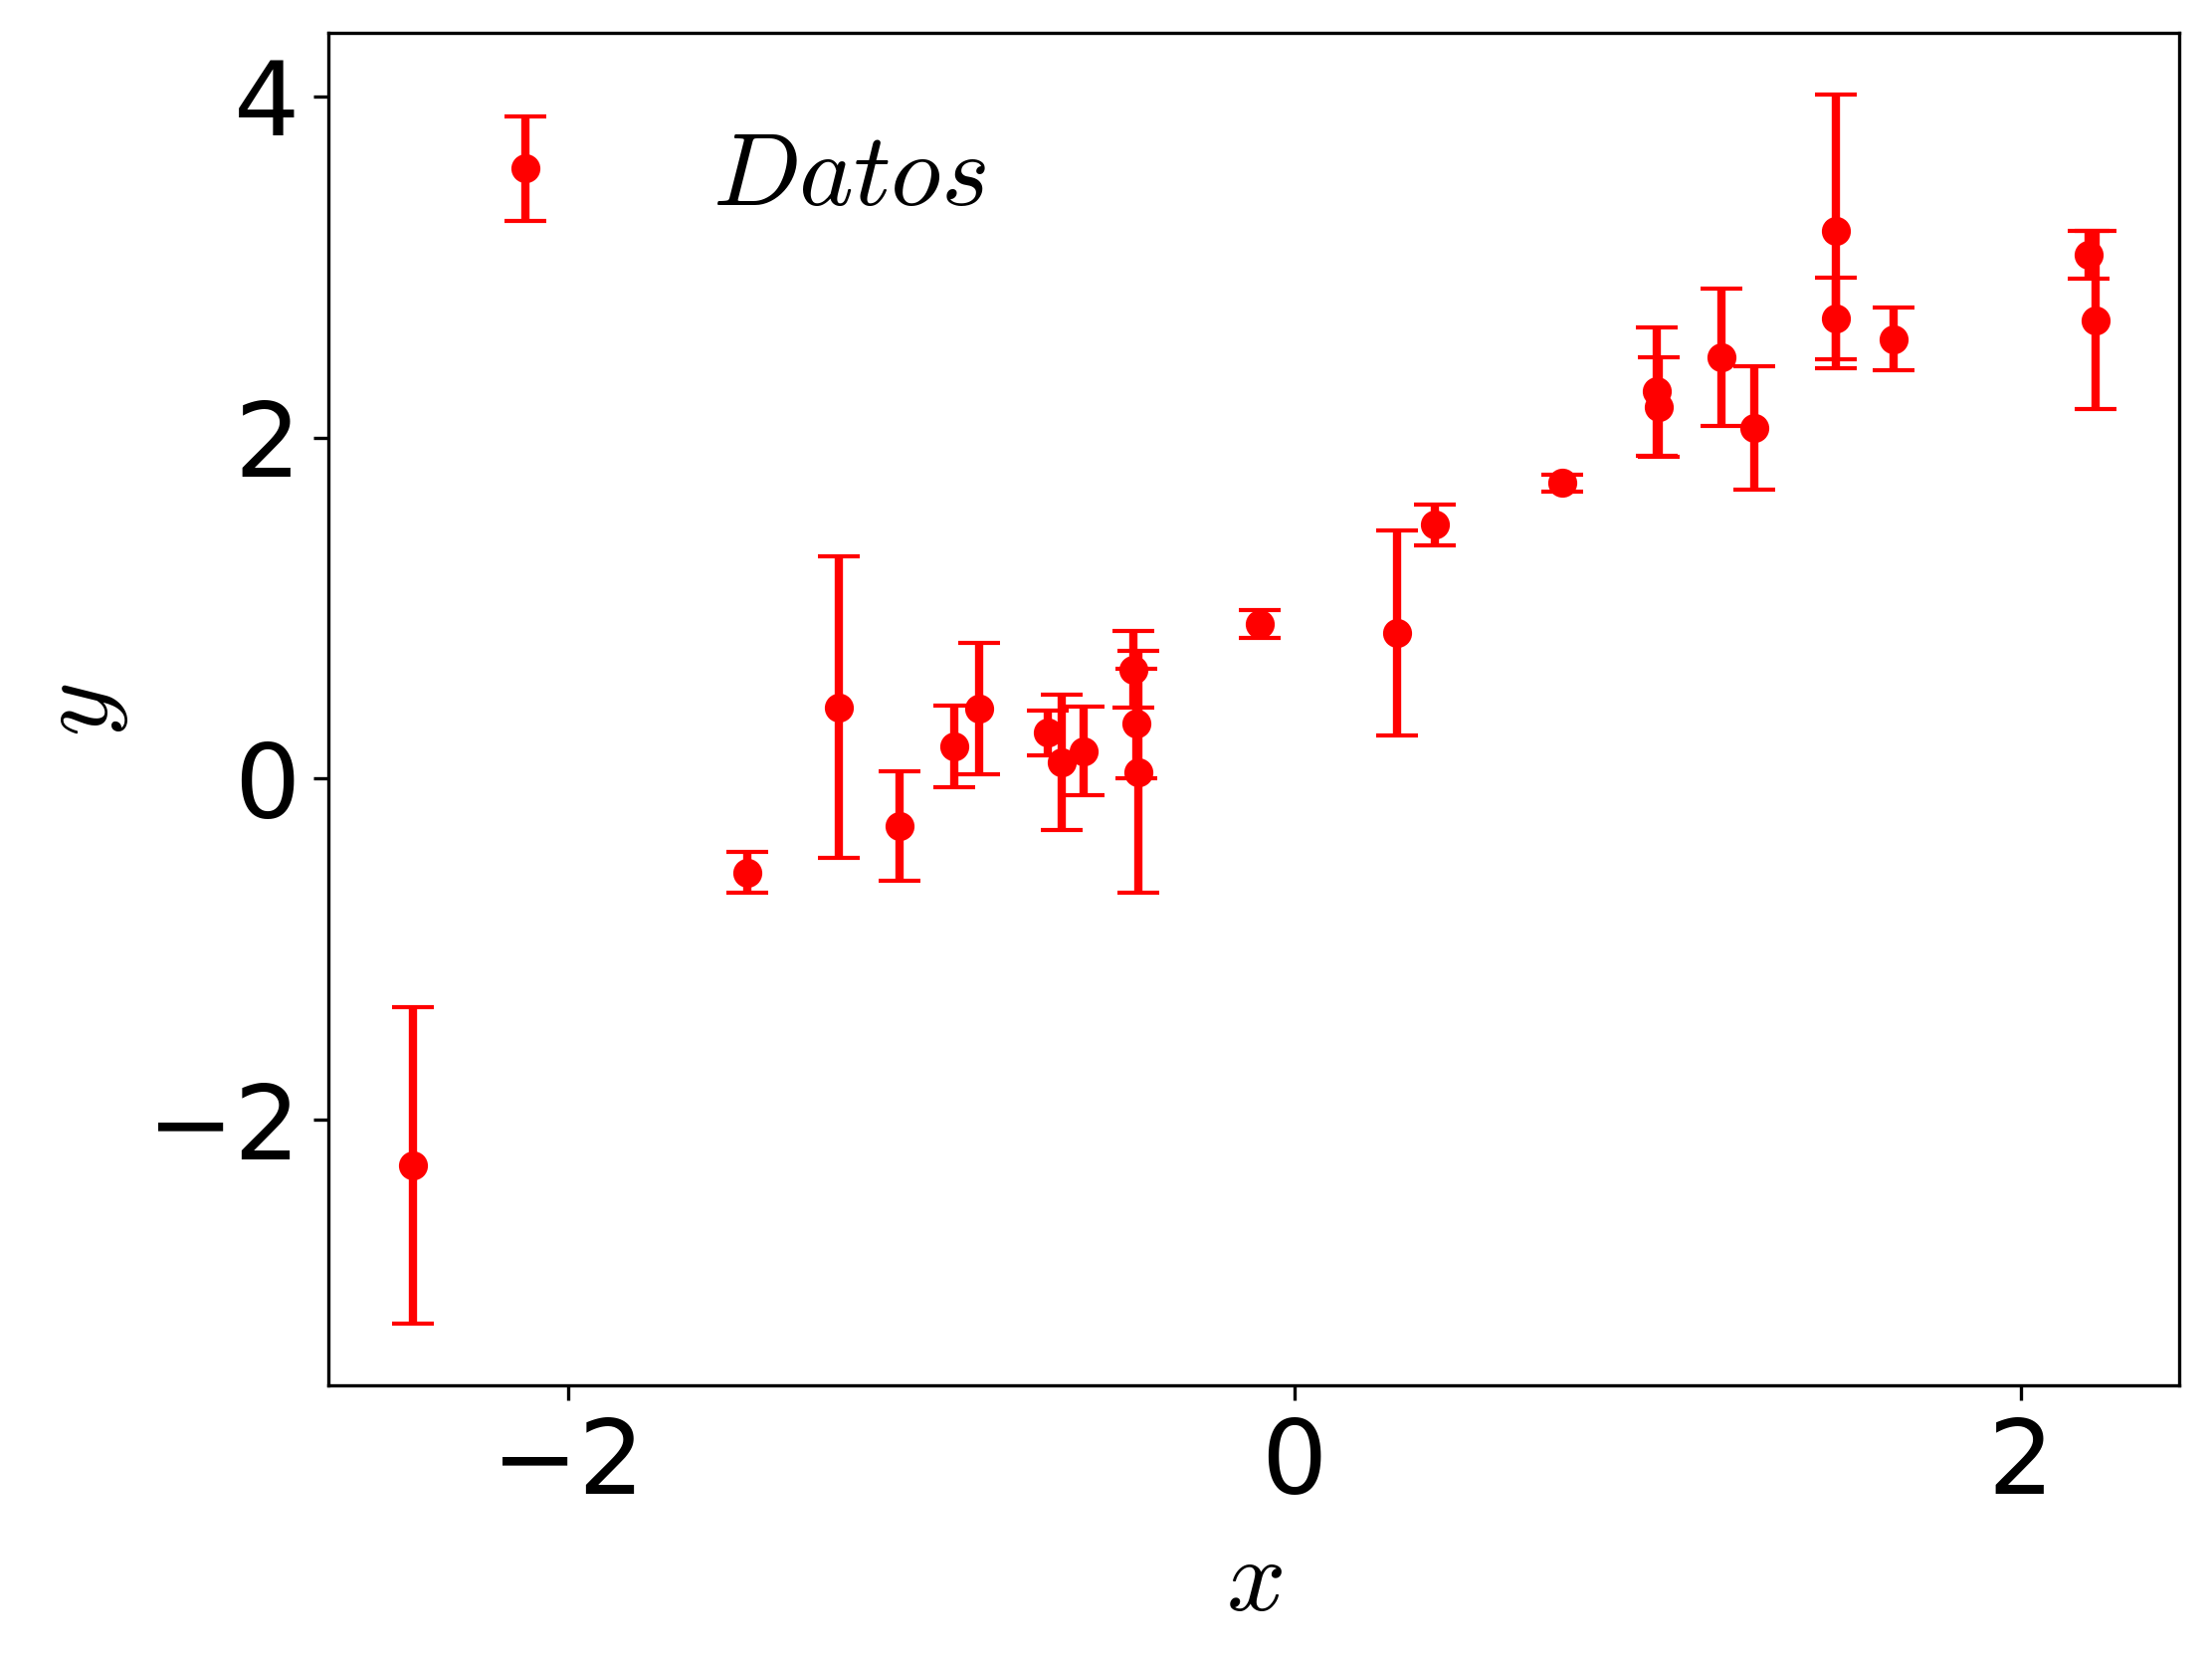
\includegraphics[height=7cm]{data.png}
\captionof{figure}{\footnotesize{Datos a lo largo de la recta $y=1+x$ con un ruido gaussiano con desviaci\'on estandar $\sigma = 0.3$.}}
\label{data}
\end{minipage}
\\

Ahora bien, supongamos que estamos interesados en conocer el valor de los par\'ametros $a$ y $m$ de nuestra recta $y=a+mx$, por lo que nos gustar\'ia estimar dichos par\'ametros mediante un proceso de inferencia Bayesiana. Tambi\'en es posible estimar cual es la desviaci\'on estandar de nuestro conjunto de datos a lo largo de la recta, lo que nos agregar\'ia un par\'ametro $\sigma$ extra por estimar. Si consideramos que en principio no conocemos nada sobre el valor de nuestros par\'ametros libres, salvo las cotas l\'imite en que \'estos deber\'ian estar, un buen prior para comenzar nuestra inferencia Bayesiana ser\'ia el considerar distribuciones planas. Para esto comenzaremos considerando los priors
\begin{equation}
a \propto U[0,1.5], \ \ \ m \propto U[0,1.5]  \ \ \ \text{y} \ \ \ \sigma \propto U[0,0.5]
\end{equation}
Considerando que existen valores de $a$, $m$ y $\sigma$ para los cuales los datos se fijan mejor (tal que el posterior es m\'aximo global), entonces de \eqref{GLik} podemos escribir el Likelihood de nuestro sistema como 
\begin{equation}
L(D;recta)\propto \exp\left[-\frac{(y_d-y)^2}{2\sigma}\right].
\end{equation}

Con esto ya podemos generar nuestras MCMC utilizando el MHA. Para \'esto hicimos uso del m\'odulo PyMC3 [ref] ya implementado en Python que nos permite emplear este m\'etodo de forma m\'as sencilla. Para el lector interesado, el c\'odigo puede encontrarse en [ref]. En nuestro an\'alisis corrimos un total de 6 cadenas con 10,000 pasos cada una. Nuestro resultado obtenido puede verse en la tabla \ref{tabla1} y la figura \ref{chain}. Como podemos ver en el lado izquierdo de la figura, existen regiones para las cuales la frecuencia de eventos en nuestro muestreo se ve incrementada. De esta manera, podemos decir que dichas regiones poseen un posterior m\'as probable para ajustarse a nuestros datos. De hecho, de la tabla \ref{tabla1} podemos observar que los valores reales para $a$ y $b$ parecen encuentrarse dentro de una desviaci\'on estandar del valor promedio estimado para estos par\'ametros, mientras que el valor real de $\sigma$ parece encuentrarse ligeramente por arriba. Adicionalmente se obtuvo el valor del criterio de convergencia de Gelman-Rubin  para cada variable con la intenci\'on de verificar que nuestros resultados obtenidos han convergido. Como podemos ver este n\'umero es muy cercano a la unidad, por lo que nuestro criterio de convergencia se cumple.

\begin{table}[h!]
\centering
\begin{tabular}{||l|l|l|l||} 
 \hline
 & \textbf{Promedio} & \textbf{Desv. Est.} & \textbf{Gelman-Rubin} \\ [0.5ex] 
 \hline\hline
$a$ & 0.957023 & 0.075513 & 0.99999 \\
\hline
$b$ & 1.059392 & 0.062649 & 1.00029\\
\hline
$\sigma$ & 0.374450 & 0.060069 & 1.00027
 \\ [1ex] 
 \hline
\end{tabular}
\caption{\footnotesize{Promedios obtenidos tras nuestra inferencia Bayesiana. Se calcula tambi\'en el criterio de Gelman-Rubin para la convergencia de las cadenas.}}
\label{tabla1}
\end{table}

\begin{minipage}{\textwidth}
\centering
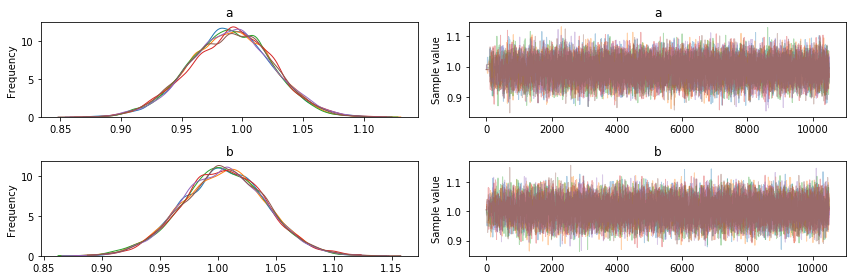
\includegraphics[height=7cm]{chain.png}
\captionof{figure}{\footnotesize{Resultados obtenidos de nuestro muestreo de pasos en nuestras cadenas de Markov.}}
\label{chain}
\end{minipage}

Como se mencion\'o, tambi\'en es importante checar si no existe autocorrelaci\'on entre las cadenas mediante las pruebas de autocorrelaci\'on. Como se puede observar en la figura \ref{autocorrplots}, conforme $lag\ k$ crece, la correlaci\'on tiende a cero, lo que nos dice que en nuestras muestras son independientes, con lo que podemos considerar que nuestro an\'alisis va bien y ha convergido completamente. 

\begin{minipage}{\textwidth}
\centering
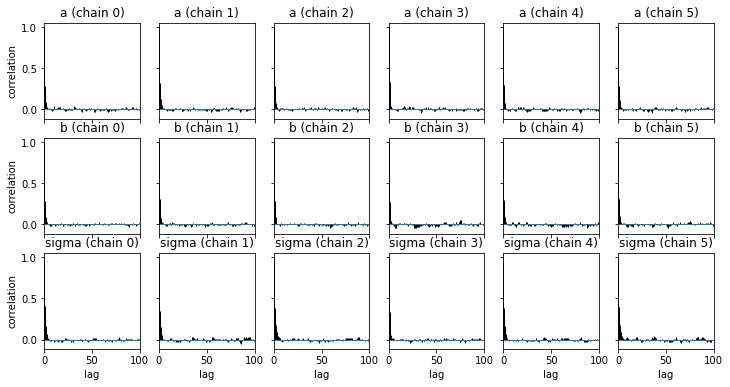
\includegraphics[height=8cm]{autocorrplots.png}
\captionof{figure}{\footnotesize{Pruebas de autocorrelaci\'on.}}
\label{autocorrplots}
\end{minipage}
\\ $ $

Finalmente s\'olo resta mostrar las t\'ipicas regiones de confidencia para nuestros par\'ametros. Las regiones que son usuales mostrar son aquellas que corresponden a un m\'ultiplo de desviaciones estandar de los par\'ametros de inter\'es. En la figura \ref{confidence} mostramos las t\'ipicas regiones de confidencia a 1-4 $\sigma$. Adem\'as hemos graficado en color rojo los valores reales de nuestros par\'ametros. Lo que podemos observar r\'apidamente es que ninguno de estos se encuentra alejado a m\'as de 2 $\sigma$s del m\'aximo estimado. Por supuesto, la raz\'on de esta discrepancia es debido a que s\'olo contamos con 25 datos para hacer nuestra inferencia Bayesiana; de contar con m\'as, nuestros resultados deber\'ian ser m\'as precisos y podr\'iamos ser capaces de acotar en una regi\'on muy peque\~na los posibles valores que nuestros par\'ametros podr\'ian tener.  

\begin{minipage}{\textwidth}
\centering
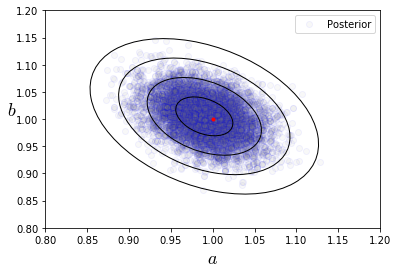
\includegraphics[height=5cm]{cab.png}\\
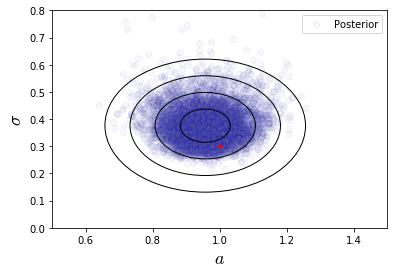
\includegraphics[height=5cm]{cas.png}
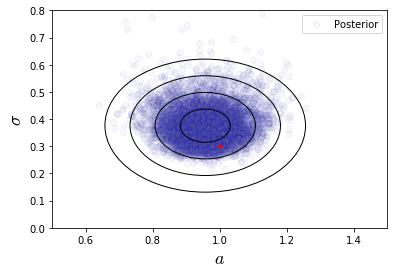
\includegraphics[height=5cm]{cas.png}
\captionof{figure}{\footnotesize{Regiones de confidencia en 2D para nuestros par\'ametros $a$, $b$ y $\sigma$. Graficamos los contornos a 1-4 $\sigma$.}}
\label{confidence}
\end{minipage}

\end{document} 
